% %% %%%%%%%%%%%%%%%%%%%%%%%%%%%%%%%%%%%%%%%%%%%%%%%%%%%%%%%%%%
% intro-control.tex
%
% Author:  Mauricio Matamoros
% License: MIT
%
% %% %%%%%%%%%%%%%%%%%%%%%%%%%%%%%%%%%%%%%%%%%%%%%%%%%%%%%%%%%%
%!TEX root = ../practica.tex
%!TEX root = ../references.bib

% CHKTEX-FILE 1
% CHKTEX-FILE 13
% CHKTEX-FILE 46

\subsection{Control}%
\label{intro-control}

Un sistema de control cerrado es aquel que utiliza un sensor para medir la salida del sistema, calcular el error respecto al valor deseado, y así suministrar la entrada necesaria para reducir el error lo más posible.
Así cuando se habla de control cerrado de manera implícita se habla de sistemas retroalimentados: aquellos en los que la salida actual depende tanto de la entrada como del error entre el valor real y el valor deseado, tal como semuestra en la \Cref{fig:closed-loop}.

\begin{figure}[H]
	\centering
	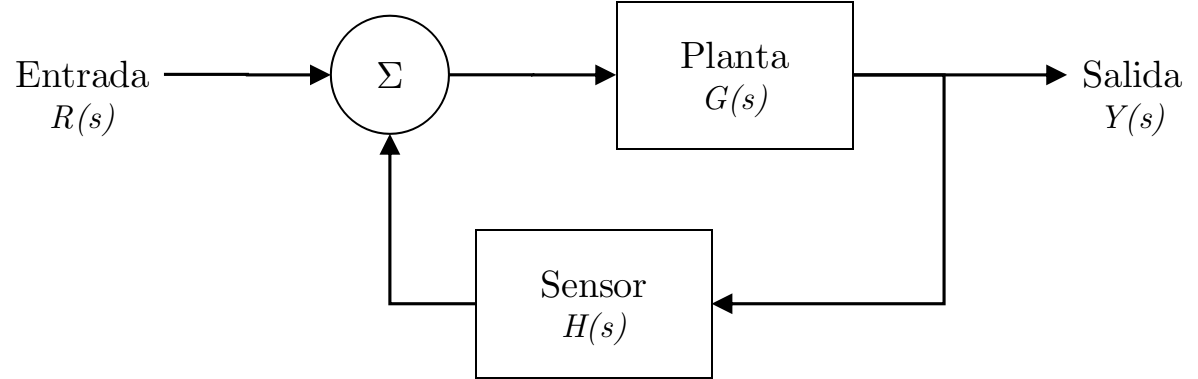
\includegraphics[width=0.8\textwidth,height=3cm,keepaspectratio]{img/closed-loop.png}
	\caption{Un sistema en lazo cerrado}%
	\label{fig:closed-loop}
\end{figure}

Para controlar un sistema con un control de lazo cerrado (en adelante \emph{sistema de control}) se necesita de tres componentes fundamentales: un sensor que convierta la salida del sistema en una señal $B(s)$ que el controlador pueda interpretar, un amplificador operacional en modo resta que calcule el error $E(s)$ entre el valor deseado o entrada $R(s)$ y el valor sensado $B(s)$, y un dispositivo controlador $G_{c}(s)$ que transforme el error $E(s)$ en la entrada $V(s)$ que necesita el sistema controlado o \emph{planta} $G_p(s)$ para producir la salida deseada $Y(s)$, tal como se ejemplifica en la \Cref{fig:control-loop}.

\begin{figure}[H]
	\centering
	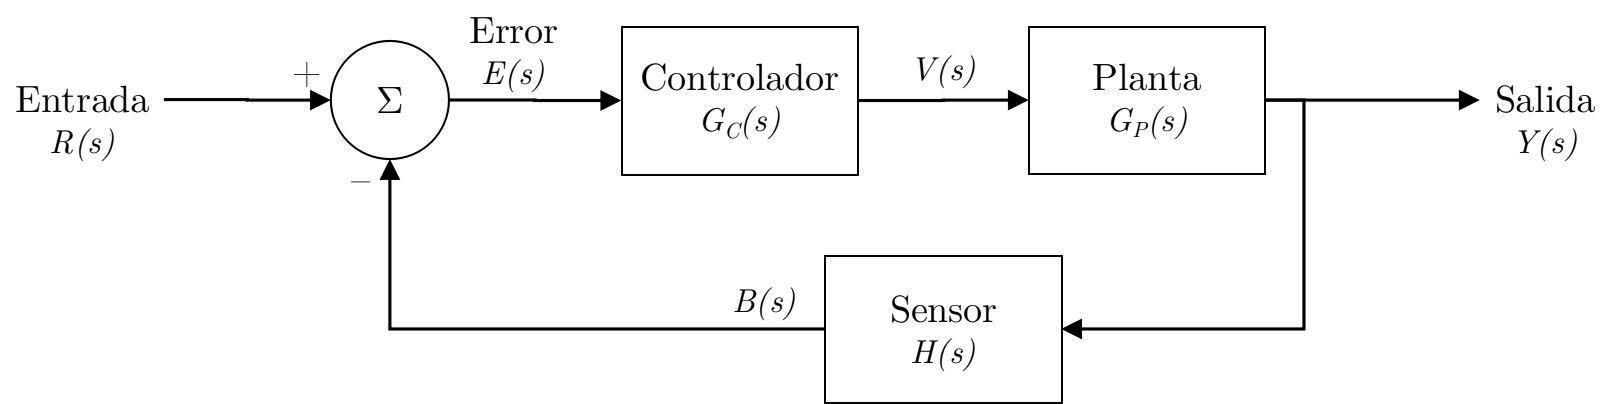
\includegraphics[width=0.8\textwidth,height=3cm,keepaspectratio]{img/control-loop.png}
	\caption{Un sistema de control en lazo cerrado}%
	\label{fig:control-loop}
\end{figure}

Debido a que los modelos de este tipo de sistemas son aproximados con funciones diferenciales, es común se utilicen transformadas como la de Laplace o Fourier para simplificar el análisis y poder modelar el controlador de forma un poco más fácil, además de que interesa mucho más conocer la respuesta en frecuencia del sistema.

Matemáticamente:

\begin{align}
	Y(s) &= E(s)G(s)%
	\tag{a}\label{eqn:sysmodel-y}\\[5pt]
	G(s) &= G_{c}(s)G_{p}(s)%
	\tag{b}\label{eqn:sysmodel-g}\\[5pt]
	E(s) &= R(s)-B(s)%
	\tag{c}\label{eqn:sysmodel-e}\\[5pt]
	B(s) &= Y(s)H(s)%
	\tag{d}\label{eqn:sysmodel-b}
\end{align}

Sustituyendo las \cref{eqn:sysmodel-e,eqn:sysmodel-g} en la \cref{eqn:sysmodel-y}:

\begin{align}
	Y(s) &= \big(G_{c}(s)G_{p}(s)\big)\big(R(s)-B(s)\big)
	\notag{}\\[5pt]%
	&= G_{c}(s)G_{p}(s)R(s)-G_{c}(s)G_{p}(s)B(s)
	\tag{e}\label{eqn:sysmodel-y2}
\end{align}

reemplazando las \cref{eqn:sysmodel-b} en la \cref{eqn:sysmodel-y2}:

\begin{align}
	Y(s) &=
		G_{c}(s)G_{p}(s)R(s)
		-
		G_{c}(s)G_{p}(s)\Big[Y(s)H(s)\Big]
	\tag{f}\label{eqn:sysmodel-y3}
\end{align}

agrupando y reordenando:
\begin{align*}
	Y(s) &=
		G_{c}(s)G_{p}(s)R(s) -
		G_{c}(s)G_{p}(s)Y(s)H(s)\\[5pt]
	Y(s) + G_{c}(s)G_{p}(s)Y(s)H(s) &=
		G_{c}(s)G_{p}(s)R(s)\\[5pt]
	Y(s)\Big[1 + G_{c}(s)G_{p}(s)H(s)\Big] &=
		G_{c}(s)G_{p}(s)R(s)\\[5pt]
	Y(s) &= \frac%
		{G_{c}(s)G_{p}(s)R(s)}%
		{1 + G_{c}(s)G_{p}(s)H(s)}\\[5pt]
\end{align*}

Con lo que finalmente se obtiene la \emph{función de transferencia de lazo cerrado} $T(s)$ para un sistema retroalimentado con control cerrado:

\begin{equation}
	T(s) = \frac{Y(s)}{R(s)} =
	\frac{G_{c}(s)G_{p}(s)}{1 + G_{c}(s)G_{p}(s)H(s)}
	\label{eqn:transfer}
\end{equation}

Esta aproximación tiene un problema fundamental: la solución analítica de este tipo de ecuaciones suele ser computacionalmente muy costoso, lo que implica que se requerirán procesadores más potentes con un mayor consumo.
Para resolver este problema, el análisis se realiza no en el contínuo, sino que se discretiza al sistema y se modela un control en tiempo discreto (o digital) usando la transformada Z.
Con este tipo de modelado, la solución de integrales se convierte en suma de valores y las diferenciales en restas, lo que reduce enormemente el costo computacional de la solución del modelo del sistema, típicamente reduciéndolo a unos cuantos productos de matrices.


% %% %%%%%%%%%%%%%%%%%%%%%%%%%%%%%%%%%%%%%%%%%%%%%%%%%%%%%%%%%%
% intro-control.tex
%
% Author:  Mauricio Matamoros
% License: MIT
%
% %% %%%%%%%%%%%%%%%%%%%%%%%%%%%%%%%%%%%%%%%%%%%%%%%%%%%%%%%%%%
%!TEX root = ../practica.tex
%!TEX root = ../references.bib

% CHKTEX-FILE 1
% CHKTEX-FILE 13
% CHKTEX-FILE 46

\subsubsection{Control On/Off}%
\label{sec:control-onoff}

Un \emph{On/Off control} o control por encendido-apagado es la técnicas de control má simple que existe.
Su principio de funcionamiento se basa en definir regiones de operación fuera de las cuales la operación de la planta se detiene.
En su versión más simple, un controlador on-off hará funcionar a la planta a máxima potencia hasta que la salida registrada supere un valor umbral (\emph{threshold}), momento en el que se reducirá la potencia de la planta, normalmente cortando el suministro de enegía o \emph{apagándola}.
La planta permanecerá apagada hasta que la salida del sistema se reduzca por debajo del umbral de operación, momento en el que el controlador volverá a poner la planta en operación a máxima potencia.

Este tipo de controlador se observa comúnmente en sistemas que responden lentamente a cambios y que tienden a almacenar mucha energía, como por ejemplo los calentadores de agua estacionarios donde el quemador se enciende hasta que la temperatura del agua se eleva hasta cierto nivel (ej.~80°C) y no se volverá a encender hasta que la temperatura registrada descienda por debajo de un umbral de operación (ej.~60°C).
Además, el mecanismo de doble umbral del calentador evita que el quemador se esté encendiendo constantemente con cambios pequeños de temperatura.

Formalmente,

\begin{equation}
V(t) =
	\begin{cases}
	r(t) & \text{si}\; \left\lvert e(t)\right\rvert \geq k\\
	0    & \text{si}\; \left\lvert e(t)\right\rvert < k\\
	\end{cases}
\end{equation}

El inconveniente principal de este tipo de controlador es que genera transiciones abruptas que tienden a desgastar los materiales, especialmente cuando se opera a altas frecuencias.
Además, con este tipo de controlador no es posible modular la entrada del sistema dentro del rango de operación, dado que las transiciones sólo se producen en los umbrales, por lo que una operación suave es imposible.
Es por esto que este tipo de controladores es raramente usado en aplicaciones industriales.

% %% %%%%%%%%%%%%%%%%%%%%%%%%%%%%%%%%%%%%%%%%%%%%%%%%%%%%%%%%%%
% intro-control-p.tex
%
% Author:  Mauricio Matamoros
% License: MIT
%
% %% %%%%%%%%%%%%%%%%%%%%%%%%%%%%%%%%%%%%%%%%%%%%%%%%%%%%%%%%%%
%!TEX root = ../practica.tex
%!TEX root = ../references.bib

% CHKTEX-FILE 1
% CHKTEX-FILE 13
% CHKTEX-FILE 46

\subsubsection{Control proporcional}%
\label{sec:control-p}
Un control es proporcional cuando la salida $v(t)$ del controlador es proporcional al error $e(t)$:
\begin{equation*}
v(t ) = K_{P} e(t)
\end{equation*}

\noindent o en el dominio de la frecuencia:

\begin{equation*}
V(s) = K_{P} E(s)
\end{equation*}

\noindent por lo tanto

\begin{equation}
G_{c}(s) = \frac{V(s)}{E(s)} = K_{P}
\label{eqn:ctrl-p}
\end{equation}

Al otorgar una señal de entrada proporcional al error, éste tipo de control opera como un amplificador de error que, al corregirse, afecta negativamente la respuesta transitoria del sistema.
Es por esto que, a pesar de que un controlador P es fácil de implementar y ajustar, suele venir acompañado de otros elementos que compensen la amplificación del error y las variaciones transitorias.

Cuando se utiliza un control proporcional~\Citep{Hernandez2010}:
\begin{itemize}[noitemsep]
	\item El tiempo de elevación experimenta una pequeña reducción.
	\item El máximo pico de sobreimpulso se incrementa.
	\item El amortiguamiento se reduce.
	\item El tiempo de asentamiento cambia en pequeña proporción.
	\item El error de estado estable disminuye con incrementos de ganancia.
	\item El tipo de sistema permanece igual.
\end{itemize}


% %% %%%%%%%%%%%%%%%%%%%%%%%%%%%%%%%%%%%%%%%%%%%%%%%%%%%%%%%%%%
% intro-control-pi.tex
%
% Author:  Mauricio Matamoros
% License: MIT
%
% %% %%%%%%%%%%%%%%%%%%%%%%%%%%%%%%%%%%%%%%%%%%%%%%%%%%%%%%%%%%
%!TEX root = ../practica.tex
%!TEX root = ../references.bib

% CHKTEX-FILE 1
% CHKTEX-FILE 13
% CHKTEX-FILE 46

\subsubsection{Control integral}%
\label{sec:control-i}
Un control es integral cuando la salida $v(t)$ del controlador es proporcional a la integral del error $e(t)$:

\begin{equation*}
v(t) = K_{I} \int e(t) dt
\end{equation*}

\noindent o en el dominio de la frecuencia:

\begin{equation*}
V(s) = \frac{K_I}{s} E(s)
\end{equation*}

\noindent por lo tanto

\begin{equation}
G_{c}(s) = \frac{V(s)}{E(s)} = \frac{K_I}{s}
\label{eqn:ctrl-i}
\end{equation}

El objetivo de un control integral es el de reducir el error de estado estable, aunque esta corrección viene a costa de sobrecorregir el error, por lo que la respuesta del sistema tiende a oscilatoria o incluso a volverse inestable.
Es por esto que un controlador I suele venir acompañado de otros elementos que ayuden a estabilizar el sistema y a reducir las oscilaciones.

Cuando se combina con un controlador tipo proporcional para formar un control PI \Citep{Hernandez2010}:
\begin{itemize}[noitemsep]
	\item El amortiguamiento se reduce.
	\item El máximo pico de sobreimpulso se incrementa.
	\item Decrece el tiempo de elevación.
	\item Se mejoran los márgenes de ganancia y fase.
	\item El tipo de sistema se incrementa en una unidad.
	\item El error de estado estable mejora por el incremento del tipo de sistema.
\end{itemize}


% %% %%%%%%%%%%%%%%%%%%%%%%%%%%%%%%%%%%%%%%%%%%%%%%%%%%%%%%%%%%
% intro-control-pd.tex
%
% Author:  Mauricio Matamoros
% License: MIT
%
% %% %%%%%%%%%%%%%%%%%%%%%%%%%%%%%%%%%%%%%%%%%%%%%%%%%%%%%%%%%%
%!TEX root = ../practica.tex
%!TEX root = ../references.bib

% CHKTEX-FILE 1
% CHKTEX-FILE 13
% CHKTEX-FILE 46

\subsubsection{Control derivativo}%
\label{sec:control-d}
Un control es derivativo cuando la salida $v(t)$ del controlador es proporcional a la derivada del error $e(t)$:

\begin{equation*}
v(t) = K_{D}\;\frac{d\;e(t)}{dt}
\end{equation*}

\noindent o en el dominio de la frecuencia:

\begin{equation*}
V(s) = K_{D}\;s\;E(s)
\end{equation*}

\noindent por lo tanto

\begin{equation}
G_{c}(s) = \frac{V(s)}{E(s)} = K_{D}s
\label{eqn:ctrl-d}
\end{equation}

Debido a que la derivada del error respecto al tiempo es la velocidad del error, un control derivativo se anticipará a los errores antes de que estos se produzcan, amortiguando oscilaciones.
Sin embargo, un controlador D es insensible a errores de estado estable, por lo que suele acompañarse de otros elementos que sí corrijan el error de estado estable.

Cuando se combina con un controlador tipo proporcional para formar un control PD \Citep{Hernandez2010}:
\begin{itemize}[noitemsep]
	\item El amortiguamiento se incrementa.
	\item El máximo pico de sobreimpulso se reduce.
	\item El tiempo de elevación experimenta pequeños cambios.
	\item Se mejoran el margen de ganancia y el margen de fase.
	\item El error de estado estable presenta pequeños cambios.
	\item El tipo de sistema permanece igual.
\end{itemize}


% %% %%%%%%%%%%%%%%%%%%%%%%%%%%%%%%%%%%%%%%%%%%%%%%%%%%%%%%%%%%
% intro-control-pid.tex
%
% Author:  Mauricio Matamoros
% License: MIT
%
% %% %%%%%%%%%%%%%%%%%%%%%%%%%%%%%%%%%%%%%%%%%%%%%%%%%%%%%%%%%%
%!TEX root = ../practica.tex
%!TEX root = ../references.bib

% CHKTEX-FILE 1
% CHKTEX-FILE 13
% CHKTEX-FILE 46

\subsubsection{Control PID digital}%
\label{sec:control-pid}
Un control \emph{proporcional-integral-derivativo} o PID incorpora las mejores características de los controles PI y PD, motivo por el cual ha sido uno de las técnicas de control continuo más utilizados en la industria por más de siete décadas \citep{Hernandez2010,Odwyer2009,Ogata2003}.

Con base en las ecuaciones \Cref{eqn:ctrl-p,sec:control-i,eqn:ctrl-d} el controlador sería de la forma:

\begin{equation}
G_{c}(s) = \frac{V(s)}{E(s)} =
	K_{P} + \frac{K_I}{s} + K_{D}s
\end{equation}

Sin embargo, como se mencionó anteriormente en la \Cref{intro-control}, integrar señales en tiempo contínuo es computacionalmente muy costoso.
Además, la señal del sensor pasará por un convertidor analógico-digital que discretizará la señal, por lo que tiene más sentido implementar un controlador discreto.
Luego entonces, interesa conocer el valor (también discreto) que se proporcionará a la planta para obtener la señal deseada en el sensor.
En el contínuo esta sería:

\begin{equation*}
v(t) = K_{P}\,e(t) + {K_I}\int e(t)\,dt+ K_{D}\frac{d\,e(t)}{dt}
\label{eqn:v-pid}
\end{equation*}

Si se muestrea el error a una intervalos de tiempo constante con frecunecia lo suficientemente alta, es posible convertir la \cref{eqn:v-pid} en una ecuación en diferencias sobre la $k$-ésima muestra tomada:

\begin{equation*}
v[k] =
		K_{P}\,e[k] +
		K_{I}\sum^{k}_{j=0} e[j]+
		K_{D}\big(e[k] - e[k-1]\big)
\end{equation*}

\noindent donde

\begin{align*}
	&e[k]                     && \text{el error actual}\\
	&e[k-1]                   && \text{el error anterior}
\end{align*}

Además, si se considera $P_{I}[k] = K_{I}\sum^{k}_{j=0} e[j]$ entonces:

\begin{align*}
P_{I}[k]
	&= K_{I}\sum^{k}_{j=0} e[j]\\
	&= K_{I}\,e[k] + P_{i}[k-1]
\end{align*}

Así, aproximar un control digital para un sistema simple puede ser tan sencillo como almacenar en memoria los últimos valores sensados del error y el acumulado de la componente integral del PID, lo que reduce el cómputo a sólo unas cuantas operaciones aritméticas simples: sumas, restas y productos.
No obstante, es necesario recordar que ésto no funcionará con sistemas que tengan una dinámica compleja, particularmente los no-lineales.



